\RequirePackage{iftex}
\ifPDFTeX
  \errmessage{This document requires XeLaTeX or LuaLaTeX. Please change your compiler.}
\fi
\documentclass[12pt]{report}

% @@@@@@@@@@@@@@@@@@@@@@@@@@@@@@@@@@@@@@@@@@@@@@@@@@@@@@@@@@@@>
% VALORES A MODIFICAR POR USTED:
% @@@@@@@@@@@@@@@@@@@@@@@@@@@@@@@@@@@@@@@@@@@@@@@@@@@@@@@@@@@@>

% NOTE: Leer nota en el README sobre la font.

\newcommand{\titulo}{Desarrollo de un pipeline basado en DRAFTS para detección y clasificación de transientes de radio con adaptación y extensión en regímenes de alta frecuencia}
\newcommand{\ciudad}{San Joaquín} % e.g. Valparaíso
% TODO: Consultar el formato de los nombres:
\newcommand{\nombrealumno}{Sebastián Salgado Polanco}
\newcommand{\nombreprofesor}{Daniela Opitz}
\newcommand{\nombrecorreferente}{Marylin Cruces}
% Mes y año del examen
\newcommand{\mesexamen}{Enero}
\newcommand{\anioexamen}{2025}
% Dedicatoria y agradecimientos
\newcommand{\dedicatoria}{
Considerando lo importancia de este trabajo para los alumnos, este apartado es para que el autor entregue palabras personales para dedicar este documento. La extensión puede ser de máximo una hoja y se deben mantener este formato, tipo y tamaño de letra.
}
\newcommand{\agradecimientos}{
Considerando la importancia de este trabajo para los alumnos, este apartado se podrá incluir en el caso de que el autor desee agradecer a las personas que facilitaron alguna ayuda relevante en su trabajo para la realización de este documento. La extensión puede ser de máximo una hoja y se deben mantener este formato, tipo y tamaño de letra.
}
\newcommand{\resumen}{
El resumen y las palabras clave no deben superar la mitad de la página, donde debe precisarse brevemente: 1) lo que el autor ha hecho, 2) cómo lo hizo (sólo si es importante detallarlo), 3) los resultados principales, 4) la relevancia de los resultados. El resumen es una representación abreviada, pero comprensiva de la memoria y debe informar sobre el objetivo, la metodología y los resultados del trabajo realizado.
}
\newcommand{\resumeningles}{
Corresponde a la traducción al idioma inglés del Resumen anterior. Sujeto a la misma regla de extensión del Resumen.
}
\newcommand{\palabrasclave}{
Cinco es el máximo de palabras clave para describir los temas tratados en la memoria, ponerlas separadas por punto y comas.
}
\newcommand{\palabrasclaveingles}{
Corresponde a la traducción al idioma inglés de Palabras Clave anteriores.
}
% @@@@@@@@@@@@@@@@@@@@@@@@@@@@@@@@@@@@@@@@@@@@@@@@@@@@@@@@@@@@>

% Paquete para importar imágenes
\usepackage{graphicx}
% Directorio de las imágenes
\graphicspath{ {figures/} }

% Idioma y fuentes
\usepackage[spanish,es-tabla]{babel}
\usepackage[T1]{fontenc}

\usepackage{fontspec}
% Selección robusta de fuente principal con respaldo en Windows
\newcommand{\MainFontName}{Carlito}
\IfFontExistsTF{Carlito}{
  \renewcommand{\MainFontName}{Carlito}
}{
  \IfFontExistsTF{Calibri}{
    \renewcommand{\MainFontName}{Calibri}
  }{
    \renewcommand{\MainFontName}{Latin Modern Roman}
  }
}
\setmainfont{\MainFontName}[BoldFont={* Bold}, ItalicFont={* Italic}]

% Paquete para definir cualquier tamaño de font
\usepackage{anyfontsize}

% Tamaño de la página y márgenes
\usepackage[letterpaper,top=2.5cm,bottom=3cm,left=3cm,right=3cm,marginparwidth=1.75cm]{geometry}

% Determinar interlineado:
\renewcommand{\baselinestretch}{1.0}

% Eliminar sangrías:
\setlength{\parindent}{0cm}

% Paquete para definir los formatos de los títulos
\usepackage[explicit]{titlesec}

\titleformat{name=\section}[block]{\fontsize{16}{24}\selectfont\bfseries}{\thesection}{0.5em}{#1}
\titleformat{name=\section,numberless}[block]{\fontsize{16}{24}\selectfont\bfseries}{}{0pt}{#1}
\titlespacing*{name=\section}{0pt}{0pt}{0.5cm}
\titlespacing*{name=\section,numberless}{0pt}{0pt}{0.5cm}

% Separación entre parrafos
\setlength{\parskip}{0.4cm}

% Paquetes de utilidad general
\usepackage{amsmath}
\usepackage{amssymb}
\usepackage{graphicx}
\usepackage{float}
\usepackage[colorlinks=true, allcolors=blue]{hyperref}

% Formato de las tablas de contenido
\usepackage{tocbasic}

%% Originalmente se usaba tocstyle en vez de tocbasic.
%% Si se quiere usar, descomentar:
% \usepackage[tocflat]{tocstyle}
% \usetocstyle{allwithdot}
%% tocstyle.sty se obtener de https://github.com/firemodels/fds/blob/master/Manuals/LaTeX_Style_Files/tocstyle.sty

% Para obtener el número de la última página
\usepackage{lastpage}

% Header y footer
\usepackage{fancyhdr}
\fancypagestyle{portada}{
    \lhead{}
    \chead{}
    \rhead{}
    \lfoot{}
    \cfoot{\fontsize{10}{12}\selectfont \thepage}
    \rfoot{}
    \renewcommand{\headrulewidth}{0pt}
}
\fancypagestyle{intermedio}{
    \lhead{}
    \chead{\fontsize{10}{12}\selectfont\MakeUppercase{\titulo}}
    \rhead{}
    \lfoot{}
    \cfoot{\fontsize{10}{12}\selectfont Página \textbf{\thepage}\ de \textbf{\pageref{LastPage}}}
    \rfoot{}
    \renewcommand{\headrulewidth}{1pt}
}

% Ajuste de altura de encabezado para evitar advertencias de fancyhdr
\setlength{\headheight}{24pt}

% Comandos para secciones
% Utilidades generales
\newcommand{\fuente}[1]{\par\small Fuente: #1}
%
% Fin utilidades
%
\newcommand{\secnumbersection}[1]{
\addtocounter{chapter}{1}
\setcounter{section}{0}
\phantomsection
\section*{CAPÍTULO \thechapter \texorpdfstring{\\}\ #1}
\addcontentsline{toc}{section}{CAPÍTULO \thechapter : #1}
\setcounter{subsection}{0}
}
\newcommand{\secnumberlesssection}[1]{
\section*{#1}
\phantomsection
\addcontentsline{toc}{section}{#1}
\setcounter{subsection}{0}
}

% Nombres
\addto\captionsspanish{\renewcommand{\contentsname}{ÍNDICE DE CONTENIDOS}}
\addto\captionsspanish{\renewcommand{\listfigurename}{ÍNDICE DE FIGURAS}}
\addto\captionsspanish{\renewcommand{\listtablename}{ÍNDICE DE TABLAS}}
\makeatletter
\renewenvironment{thebibliography}[1]
     {\secnumberlesssection{REFERENCIAS BIBLIOGRÁFICAS}
      \@mkboth{\MakeUppercase\bibname}{\MakeUppercase\bibname}%
      \list{\@biblabel{\@arabic\c@enumiv}}%
           {\settowidth\labelwidth{\@biblabel{#1}}%
            \leftmargin\labelwidth
            \advance\leftmargin\labelsep
            \@openbib@code
            \usecounter{enumiv}%
            \let\p@enumiv\@empty
            \renewcommand\theenumiv{\@arabic\c@enumiv}}%
      \sloppy
      \clubpenalty4000
      \@clubpenalty \clubpenalty
      \widowpenalty4000%
      \sfcode`\.\@m}
     {\def\@noitemerr
       {\@latex@warning{Empty `thebibliography' environment}}%
      \endlist}
\makeatother

% Personalizar Tabla de Contenidos

\usepackage{tocloft}
\renewcommand{\cftsecfont}{\fontsize{12}{14}\selectfont\fontspec{\MainFontName}}
\renewcommand{\cftsubsecfont}{\fontsize{12}{14}\selectfont\fontspec{\MainFontName}}
\renewcommand{\cftsubsubsecfont}{\fontsize{12}{14}\selectfont\fontspec{\MainFontName}}

\renewcommand\cftfigfont{\fontsize{12}{14}\selectfont\fontspec{\MainFontName}}

% Links sin color
\usepackage{hyperref}
\hypersetup{colorlinks = false}

% Comando para secciónes sin enumeración
% (sugerido por @anibalbastiass https://github.com/autopawn/tex-thesis-template/issues/5#issuecomment-916106128)
\newcommand{\secnumberlesssubsection}[1]{
\subsection*{#1}
\phantomsection
\addcontentsline{toc}{subsection}{#1}
\setcounter{subsection}{0}
}
% Forma de uso:
% \secnumberlesssubsection{"Sub seccion sin enumeración"}

% @@@@@@@@@@@@@@@@@@@@@@@@@@@@@@@@@@@@@@@@@@@@@@@@@@@@@@@@@@@@>
\begin{document}
\sloppy % Para evitar que referencias se escapen de los márgenes.

\pagestyle{portada}
\pagenumbering{roman}
% NOTE: Este archivo contiene la portada, la dedicatoria, los agradecimientos y el resumen.
% __NO ES NECESARIO MODIFICAR ESTE ARCHIVO__, esas se modifican con los comandos que aparecen en main.tex
%@@@@@@@@@@@@@@@@@@@@@@@@@@@@@@@@@@@@@@@@@@@@@@@@@@@@@@@@@@@@@@
\begin{titlepage}
\begin{center}
\noindent
{\fontsize{18}{22}\selectfont UNIVERSIDAD TÉCNICA FEDERICO SANTA MARÍA \\}
{\fontsize{16}{19}\selectfont DEPARTAMENTO DE INFORMÁTICA \\}
{\fontsize{16}{19}\selectfont \MakeUppercase{\ciudad}\ - CHILE \\}
\vspace{1.5cm}

\includegraphics[width=4.41cm,height=3.34cm]{logo/logo.jpg} \\
\vspace{1.5cm}
{\fontsize{20}{24}\selectfont ``\MakeUppercase{\titulo}'' \\}
\vfill
{\fontsize{16}{19}\selectfont \MakeUppercase{\nombrealumno} \\}
\vfill
{\fontsize{16}{19}\selectfont MEMORIA PARA OPTAR AL TÍTULO DE \\}
{\fontsize{16}{19}\selectfont INGENIERO CIVIL EN INFORMÁTICA \\}
\vspace{1.5cm}
{\fontsize{14}{17}\selectfont Profesor Guía: \nombreprofesor \\}
{\fontsize{14}{17}\selectfont Profesor Correferente: \nombrecorreferente \\}
\vspace{2.5cm}
{\fontsize{14}{17}\selectfont \mesexamen\ - \anioexamen \\}
\end{center}
\end{titlepage}

%@@@@@@@@@@@@@@@@@@@@@@@@@@@@@@@@@@@@@@@@@@@@@@@@@@@@@@@@@@@@@@
\newpage
\setcounter{page}{2}
\
\vfill
\vfill
\begin{flushright}
\noindent {\fontsize{16}{19}\selectfont \textbf{DEDICATORIA} \\}
\end{flushright}
\begin{flushright}
\noindent \dedicatoria
\end{flushright}
\vfill
%@@@@@@@@@@@@@@@@@@@@@@@@@@@@@@@@@@@@@@@@@@@@@@@@@@@@@@@@@@@@@@
\newpage
\begin{center}
\noindent {\fontsize{16}{19}\selectfont \textbf{AGRADECIMIENTOS} \\}
\end{center}
\noindent \agradecimientos
\vfill
%@@@@@@@@@@@@@@@@@@@@@@@@@@@@@@@@@@@@@@@@@@@@@@@@@@@@@@@@@@@@@@
\newpage
\secnumberlesssection{RESUMEN}
\vspace{0.3cm}
\noindent \textbf{Resumen---}\resumen \ \\
\vspace{0.3cm} \\
\noindent \textbf{Palabras Clave---}\palabrasclave \ \\
% @@@@@
\vspace{1.2cm} \\
% @@@@@
%\noindent {\fontsize{16}{19}\selectfont \textbf{ABSTRACT}}
%\vspace{1.2cm} \\
\secnumberlesssection{ABSTRACT}
\vspace{0.3cm}
\noindent \textbf{\emph{Abstract}---}\resumeningles \ \\
\vspace{0.3cm} \\
\noindent \textbf{\emph{Keywords}---}\palabrasclaveingles \ \\
%@@@@@@@@@@@@@@@@@@@@@@@@@@@@@@@@@@@@@@@@@@@@@@@@@@@@@@@@@@@@@@


\newpage
\secnumberlesssection{GLOSARIO}

Aquí se deben colocar las siglas mencionadas en el trabajo y su explicación, por orden alfabético. Por ejemplo: \\

{\setlength{\parskip}{0cm} % Para evitar saltar entre cada elemento nombrado.
%Colocar aquí siglas:
DI: Departamento de Informática.

UTFSM: Universidad Técnica Federico Santa María.
}


%Índice de contenidos:
\newpage
\thispagestyle{portada}
\tableofcontents

%Índice de figuras:
\newpage
\thispagestyle{portada}
\phantomsection
\addcontentsline{toc}{section}{ÍNDICE DE FIGURAS}
\listoffigures
\phantomsection
\addcontentsline{toc}{section}{ÍNDICE DE TABLAS}
\listoftables

\newpage
\pagestyle{intermedio}
\pagenumbering{arabic}
\secnumbersection{INTRODUCCIÓN}

\section{Contexto y motivación}
En la última década, la radioastronomía ha revelado la existencia de fenómenos transitorios extremadamente breves y energéticos, entre los que destacan las \textit{ráfagas rápidas de radio} (Fast Radio Bursts, FRBs). Las FRBs son pulsos de emisión de radio de duración del orden de milisegundos, generalmente originados a distancias extragalácticas. Su descubrimiento inicial en 2007 marcó un hito por la intensidad y lejanía de estas señales \cite{Lorimer_2007}. El estudio de las FRBs es de gran relevancia científica: estas ráfagas pueden utilizarse como trazadores del medio intergaláctico, aportando información sobre la distribución de materia bariónica y sobre campos magnéticos a escalas cosmológicas, además de ofrecer nuevas oportunidades para la cosmología observacional \cite{Petroff_2022}. 

\begin{figure}[h]
\centering
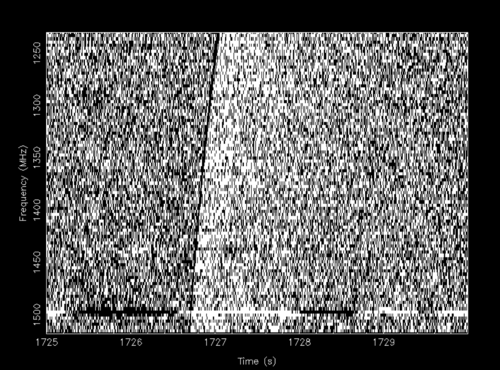
\includegraphics[width=0.8\textwidth]{figures/Lorimer Burst.png}
\caption{Ráfaga de Lorimer: observación de la primera ráfaga de radio rápida detectada, tal como la describió Lorimer en 2006.}
\label{fig:lorimer}
\end{figure}

\section{Problema}
Detectar FRBs en tiempo de procesamiento plantea desafíos considerables. Los radiotelescopios modernos generan volúmenes masivos de datos, lo que dificulta el procesamiento eficiente de observaciones en busca de eventos de milisegundos. A esto se suma la abundante interferencia de radiofrecuencia (RFI) de origen humano, que contamina las señales e imita pulsos astrofísicos, produciendo grandes listas de candidatos falsos. Los métodos tradicionales de búsqueda de pulsos individuales como los algoritmos implementados en suites clásicas tipo PRESTO y Heimdall se basan en dedispersión exhaustiva y umbrales fijos de detección, si bien han sido exitosos, son propensos a listas extensas de falsos positivos y requieren inspección manual intensiva, lo que limita su uso en operación en tiempo (casi) real \cite{Cordes_2003, Ransom_2003, Barsdell_2012}. Por otra parte, \textbf{DRAFTS} aporta modelos de detección y clasificación, pero no un pipeline operativo extremo a extremo.

\textbf{TODO (Problema específico)}: Completar con 3–4 frases que describan el vacío exacto en tu contexto (datos disponibles, limitaciones de herramientas actuales en tu entorno, necesidad de near-real-time, etc.).

\section{Objetivos}
\textbf{Objetivo general:} Diseñar e implementar un pipeline basado en DRAFTS para detección y clasificación de transientes de radio, y extenderlo a regímenes de alta frecuencia.\\
\textbf{Objetivos específicos:}
\begin{itemize}
  \item Integrar y operacionalizar los modelos de DRAFTS en un pipeline reproducible.
  \item Diseñar módulos de ingesta, preprocesado, detección, clasificación y reporte.
  \item Adaptar la búsqueda a frecuencias milimétricas (mm-wave) considerando sus particularidades.
  \item Evaluar desempeño (recall, precision, F1, latencia) en banda L y en mm-wave.
\end{itemize}

\textbf{TODO (Medición de objetivos)}: Indicar cómo verificarás cada objetivo (p.ej., latencia \(<\) N s/archivo de 32 GB; F1 \(>\) X en FRB121102).

\section{Preguntas de investigación e hipótesis}
¿Cómo se comporta la detección y clasificación de FRBs al comparar banda L con mm-wave? Hipótesis: la atenuación del patrón bow-tie en mm-wave disminuye sensibilidad de detectores basados en tiempo–DM, mitigable ampliando rango/step de DM y mediante validación por sub-bandas y clasificación a DM\(\approx 0\).

\textbf{TODO (Criterios de falsación)}: Expresar qué resultados refutarían/confirmarían la hipótesis (p.ej., recall relativo mm-wave/L-band, tasa de falsos DM\(\approx\)0).

\section{Principales contribuciones técnicas}
\begin{itemize}
  \item Pipeline DRAFTS-MB con módulos definidos, contratos I/O y configuración.
  \item Estrategias de chunking/slices/overlap con criterios formales de \(\Delta DM\) por smearing.
  \item Integración CenterNet (detección) + ResNet (clasificación) con umbrales robustos (MAD/IQR).
  \item Extensión y validación en mm-wave y lineamientos para operación near-real-time.
\end{itemize}

\textbf{TODO (Evidencias de contribución)}: Enumerar outputs verificables (scripts, configs, artefactos, figuras clave, IDs de commit).

\section{Alcance y limitaciones}
El trabajo se enfoca en búsqueda de pulsos individuales (single-pulse) y no aborda timing ni localización interferométrica plena. Se trabaja con PSRFITS/FIL, con disponibilidad de GPU estándar. Limitaciones incluyen RFI a DM\(\approx 0\), dependencia de metadatos fiables y variabilidad instrumental.

\textbf{TODO (Límites explícitos)}: Añadir supuestos concretos (p.ej., resolución temporal mínima, anchos de banda soportados, formatos exactos, versiones de librerías).

\section{Organización del documento}
Este documento se organiza en diez capítulos más anexos. El Capítulo 2 presenta el marco teórico; el 3, el estado del arte; el 4, los requisitos y el diseño del pipeline; el 5, la implementación; el 6, la metodología experimental y los datasets; el 7, los resultados en banda L; el 8, la extensión a mm-wave (ALMA); el 9, la discusión y amenazas a la validez; y el 10, las conclusiones y trabajo futuro.

\section{Posicionamiento frente a pipelines en tiempo real}
Como motivación y punto de comparación, se discuten arquitecturas operativas de CHIME/FRB, ASKAP/CRAFT y MeerTRAP, destacando diferencias en adquisición, backend, mitigación de RFI y criterios de decisión, que orientan los requisitos y decisiones del presente pipeline.

\newpage
\secnumbersection{MARCO TEÓRICO}

\section{FRBs y pulsos individuales: DM, dispersión, ancho y S/N}
Las FRBs son pulsos de duración típica de milisegundos, caracterizados por su \textit{Medida de Dispersión} (DM), ancho intrínseco/observado y relación señal/ruido (S/N). La dispersión en el medio ionizado introduce un retardo en frecuencia que se aproxima por
\[\Delta t\,\,\mathrm{[ms]} \approx 4.15\times10^3\,\mathrm{DM}\,\left(\nu_1^{-2}-\nu_2^{-2}\right),\]
donde \(\nu\) se expresa en MHz. El ensanchamiento por dispersión y efectos instrumentales (\textit{smearing}) limita la sensibilidad si excede el ancho del pulso.

\section{Plano tiempo--DM y patrón ``bow-tie''}
La búsqueda de pulsos individuales se realiza en el plano tiempo--DM, donde una ráfaga astrofísica genera un patrón en ``corbatín'' (\textit{bow-tie}). La apertura del patrón depende de la cobertura en frecuencia y de la DM del evento; el máximo S/N aparece cerca de la DM verdadera.

\section{RFI: criterios de discriminación astrofísico vs terrestre}
La RFI suele concentrarse en bandas estrechas, presenta DM cercana a cero y carece de la dispersión cromática propia de señales cósmicas. Criterios como consistencia en sub-bandas, simetría temporal, estabilidad de DM y persistencia espacial ayudan a discriminar eventos astrofísicos.

\section{Dedispersión y waterfalls (sin y con dedispersión)}
Los \textit{waterfalls} crudos muestran la dispersión en frecuencia; tras dedispersar a una DM candidata, un pulso real se alinea temporalmente a través de canales. La inspección conjunta tiempo--DM y \textit{waterfalls} dedispersados es clave para validar candidatos.

\section{Particularidades a alta frecuencia (mm-wave)}
A frecuencias milimétricas el retardo por dispersión es menor, atenuando el ``bow-tie'' y reduciendo la ganancia de S/N asociada a la dedispersión. Esto exige ampliar el rango y el paso de DM o estrategias de validación por sub-bandas y clasificación complementaria.

\section{Telescopios y datos relevantes}
Se consideran instrumentos y formatos representativos: FAST y Effelsberg (banda L), y ALMA en modo \textit{phased} para frecuencias milimétricas. Formatos habituales: PSRFITS/SEARCH y \texttt{FIL}, con metadatos esenciales como \texttt{TBIN}, \texttt{NCHAN}, ancho de banda, frecuencias y tiempos de inicio en MJD.

\section{Convenciones de polarización (PSR/IEEE) y PSRFITS/PSRCHIVE}
Se adopta la convención PSR/IEEE para Stokes \(I,Q,U,V\). La correcta interpretación y almacenamiento de polarización en PSRFITS y su tratamiento en PSRCHIVE son relevantes para análisis avanzados y mitigación de RFI.

\section{Trazabilidad temporal}
Se resguarda trazabilidad mediante sellos de tiempo absolutos (MJD topocéntrico) y consistencia con modelos temporales (p.ej., TEMPO2), asegurando coherencia entre bloques y reproductibilidad de ventanas temporales.

\newpage
\secnumbersection{ESTADO DEL ARTE}

\section{Pipelines y herramientas de búsqueda de pulsos}
Se revisan suites como PRESTO y Heimdall, y otras herramientas relevantes para búsquedas de pulsos individuales, destacando fortalezas y limitaciones en escenarios operativos.

\textbf{TODO}: Añadir referencias y una tabla breve comparando PRESTO vs Heimdall vs otros (entradas, desempeño, salida, facilidad de integración).

\section{DRAFTS: detector CenterNet y clasificador ResNet}
Se describe el enfoque DRAFTS, su arquitectura de detección en tiempo--DM y la clasificación binaria, explicitando qué resuelve y qué queda fuera del alcance (pipeline operativo extremo a extremo).

\textbf{TODO}: Resumir hiperparámetros y tamaños de entrada de los modelos de DRAFTS empleados.

\section{Estudios a frecuencias altas}
Se resumen intentos y hallazgos en bandas altas, identificando brechas y desafíos abiertos.

\textbf{TODO}: Incorporar 1–2 trabajos recientes en mm-wave y su pertinencia para ALMA.

\section{Síntesis del gap abordado}
Se articula el vacío entre modelos de ML y su operacionalización, y la extensión a mm-wave propuesta en este trabajo.

\section{Arquitecturas operativas: CHIME/FRB, ASKAP/CRAFT, MeerTRAP}
Se reseñan arquitecturas en tiempo real/\textit{near-real-time}, mecanismos de backend y publicación de candidatos, como referencia para requerimientos y comparación.

\textbf{TODO}: Esbozar 4–5 bullets por arquitectura con su pipeline y latencias.

\section{Mitigación de RFI}
Panorama de estrategias aceptadas (AOFlagger, enfoques morfológicos/estadísticos) y su relación con el preprocesado del pipeline.



\newpage
\secnumbersection{REQUISITOS Y DISEÑO (ALTO NIVEL) DEL PIPELINE DRAFTS-MB}

\section{Requisitos funcionales del pipeline (qué debe cumplir)}
Ingesta, preprocesado, detección, clasificación, visualización, reporte y trazabilidad, con configuración reproducible.

\textbf{TODO (qué completar aquí)}: Detallar por módulo: entradas (formatos, tamaños), salidas (artefactos/figuras/tablas), contratos (JSON/YAML), y 1 ejemplo mínimo end-to-end (archivo→candidatos→figuras).

\section{Requisitos no funcionales (latencia, RAM, reproducibilidad)}
Operación en tiempo real/\textit{near-real-time}, uso de RAM y reproducibilidad controlada (semillas, versiones, contenedores).

\textbf{TODO (parámetros objetivo)}: Fijar límites de latencia por archivo/bloque, tope de RAM y CPU/GPU; incluir política de semillas/versionado (manifest con commit/pesos/entorno) y criterio de éxito.

\section{Arquitectura: módulos, flujos y contratos (diseño de alto nivel)}
Arquitectura en cinco fases: (1) ingesta de datos, (2) preprocesamiento, (3) procesamiento (detección y clasificación), (4) visualización, (5) resultados y registro. 
Definición de módulos, interfaces I/O, configuración, registro (logging) y manejo de errores. Los modelos se usan como APIs consumibles para aislar dependencias.

\textbf{TODO (diagrama)}: Bocetar las conexiones entre módulos (puertos/interfaces) y definir estados de error/retentos (qué hacer ante fallas parciales y reintentos).

\section{Modelo de datos y trazabilidad temporal (timestamps y ventanas)}
Timestamps absolutos (MJD), ventanas de visualización y metadatos mínimos para reproducibilidad.

\textbf{TODO (checklist)}: Enumerar metadatos obligatorios por bloque (MJD, frecuencia de referencia, TBIN, NCHAN, ancho de banda, identificador de backend) y cómo se validan/coinciden entre ejecuciones.

\subsection*{Notación y variables}
\begin{description}
  \item[$\mathrm{DM}$] Medida de dispersión (pc\,cm$^{-3}$); $k_{\mathrm{DM}}=4.1488\times10^3$\,ms\,MHz$^{2}$\,pc$^{-1}$\,cm$^{3}$.
  \item[$\nu_{\min},\,\nu_{\max},\,\nu_{\mathrm{ref}}$] Frecuencias (MHz) mínima, máxima y de referencia; $\nu_c$ es la del canal $c$.
  \item[$\Delta\nu$] Ancho de canal en MHz; $\nu_{\mathrm{GHz}}$ es la frecuencia en GHz.
  \item[$\Delta t$] Resolución temporal (ms); $\Delta t_{\mathrm{samp}}$ resolución de muestreo.
  \item[$W,\,\tau_{\mathrm{sc}},\,\tau_{\mathrm{chan}}$] Ancho intrínseco y ensanchamientos por scattering y canal.
  \item[$D,\,C,\,S,\,N$] Nº de DM, canales, muestras por slice y muestras totales en tiempo.
  \item[$H\times W$] Tamaño de entrada del detector; $E_{\mathrm{det}},\,E_{\mathrm{cls}}$ costos de inferencia.
  \item[$\alpha,\,\beta$] Constantes de costo (dedispersión, extracción de rasgos/peaks).
  \item[$O$] Solapamiento (muestras) entre ventanas; $B,\,B'$ nº de candidatos por slice (ramas main/HF).
\end{description}

\section{Estrategias de performance (chunking/slicing/overlap/decimado)}
Procesamiento por \textit{chunks} y \textit{slices} con \textit{overlap}, gestión de memoria y paralelismo. Diseño consciente de RAM: coordinación chunk--slice, solapamiento entre chunks para evitar pérdidas en bordes por rangos de DM, y controles de resolución/decimado ajustables por el usuario.

\textbf{TODO (valores guía)}: Proponer valores por defecto y rangos recomendados para chunk, slice, overlap y decimados; justificar según ecuaciones de smearing y presupuesto de memoria.

\subsection*{Notas sobre S/N y decimado}
Relación S/N (aprox.) al sumar muestras/canales tras dedispersión:
\begin{equation}\label{eq:snr_scaling}
\mathrm{SNR}\ \propto\ \frac{A}{\sigma}\,\sqrt{N_{\mathrm{sum}}}.
\end{equation}

Elección de decimado \(k\) y filtro tipo boxcar:
\begin{equation}\label{eq:weff_decimation}
W_{\mathrm{eff}}\ \approx\ k\,\Delta t_{\mathrm{samp}},\quad \text{maximizar S/N con ancho de filtro} \ \approx W_{\mathrm{eff}}.
\end{equation}

\section{Criterios formales: paso de DM por smearing (diseño de $\Delta$DM/overlap)}
Se definen pasos de DM y \textit{overlap} mínimo con base en preservar el S/N de pulsos de ancho \(W\). Una relación práctica es mantener el ensanchamiento por dispersión inferior al ancho objetivo.

\textbf{TODO (ejemplo numérico)}: Aplicar las fórmulas a tu banda (\(\nu_{\min},\nu_{\max}\)), TBIN y ancho objetivo \(W\) para derivar \(\Delta\mathrm{DM}\) y overlap mínimos; incluir un caso de referencia.

\subsection*{Ecuaciones relevantes}
Retardo de dispersión entre dos frecuencias (\(\nu\) en MHz):
\begin{equation}\label{eq:dm_delay_band}
\Delta t_{\mathrm{DM}}\,[\mathrm{ms}] \approx 4.1488\times10^{3}\,\mathrm{DM}\,\big(\nu_1^{-2}-\nu_2^{-2}\big).
\end{equation}

Smearing intra-canal (\(\nu\) en GHz, \(\Delta\nu\) en MHz):
\begin{equation}\label{eq:smear_intrach}
\tau_{\mathrm{smear}}\,[\mu\mathrm{s}] \approx 8.3\,\mathrm{DM}\,\frac{\Delta\nu_{\mathrm{MHz}}}{\nu_{\mathrm{GHz}}^{3}}.
\end{equation}

Error por DM desajustada en la banda \([\nu_{\min},\nu_{\max}]\):
\begin{equation}\label{eq:dm_error}
\tau_{\mathrm{err}}(\Delta\mathrm{DM})\,[\mathrm{ms}] \approx 4.1488\,\Delta\mathrm{DM}\,\big(\nu_{\min}^{-2}-\nu_{\max}^{-2}\big).
\end{equation}

Condición de diseño para el paso de DM (con \(f\in[0.2,0.5]\)):
\begin{equation}\label{eq:dm_step_criterion}
\tau_{\mathrm{err}}(\Delta\mathrm{DM})\ \le\ f\,W_{\mathrm{eff}}\ \Rightarrow\ \Delta\mathrm{DM}\ \le\ \frac{f\,W_{\mathrm{eff}}}{4.1488\,\big(\nu_{\min}^{-2}-\nu_{\max}^{-2}\big)}.
\end{equation}

Solape mínimo entre \textit{chunks}:
\begin{equation}\label{eq:overlap_min}
\mathrm{overlap}_{\min}\ \ge\ \Delta t_{\mathrm{DM}}\big(\mathrm{DM}_{\max\ \mathrm{ventana}}\big)\ +\ \mathrm{margen}_{\mathrm{filtro}}.
\end{equation}

\section{Control del trials factor y tasas de error (FAR/FPR)}
Estimación del \textit{trials factor} en el plano DM\(\times\)tiempo y definición preliminar de FAR/FPR para la toma de decisiones.

\textbf{TODO (umbrales)}: Especificar FAR/h objetivo y derivar el umbral \(z\) asociado (con \(N_{\mathrm{trials/h}}\)); documentar impacto en recall/precision.

\subsection*{Ecuaciones relevantes}
Número de pruebas aproximado:
\begin{equation}\label{eq:ntrials}
N_{\mathrm{trials}}\ \approx\ N_{\mathrm{DM}}\,N_{\mathrm{tiempo}}\,N_{\mathrm{anchos}}.
\end{equation}

Para ruido gaussiano, probabilidad de falso por prueba con umbral \(z\):
\begin{equation}\label{eq:qfunc}
p_0\ \approx\ Q(z),\quad Q(z)=\tfrac{1}{\sqrt{2\pi}}\int_{z}^{\infty}\!e^{-u^2/2}\,du.
\end{equation}

Tasa de falsas alarmas por hora (FAR) y elección de \(z\):
\begin{equation}\label{eq:far}
\mathrm{FAR}\ \approx\ N_{\mathrm{trials/h}}\,p_0\ \Rightarrow\ z\ =\ Q^{-1}\!\Big(\tfrac{\mathrm{FAR}}{N_{\mathrm{trials/h}}}\Big).
\end{equation}

\section{DM--tiempo y dedispersión (fundamentos)}
\noindent \textbf{Retardo por canal} respecto de una referencia \(\nu_{\mathrm{ref}}\) (frecuencias en MHz):
\begin{equation}\label{eq:delta_t_dm_ref}
\Delta t_{\mathrm{DM}}(c;\,\mathrm{DM})\,[\mathrm{ms}] = 4.1488\times10^{3}\,\mathrm{DM}\,\big(\nu_c^{-2} - \nu_{\mathrm{ref}}^{-2}\big).
\end{equation}
\noindent \textbf{Transformación temporal:}
\begin{equation}\label{eq:tprime}
t' = t + \Delta t_{\mathrm{DM}}(c;\,\mathrm{DM}).
\end{equation}
\noindent \textbf{Cubo tiempo--DM (suma en frecuencia):}
\begin{equation}\label{eq:cube_sum}
X(d,t) = \sum_{c=1}^{C} x\!\left(c,\ t - \frac{\Delta t_{\mathrm{DM}}(c;\,\mathrm{DM}_d)}{\Delta t}\right).
\end{equation}
\noindent \textbf{Ancho efectivo del pulso:}
\begin{equation}\label{eq:weff}
W_{\mathrm{eff}}^2 = W^2 + \tau_{\mathrm{sc}}^2 + \tau_{\mathrm{chan}}^2,\qquad \tau_{\mathrm{chan}} \approx 4.1488\,\mathrm{ms}\,\mathrm{DM}\,(\nu_{\min}^{-2}-\nu_{\max}^{-2}).
\end{equation}
\noindent \textbf{Espaciado de DM} (pérdida \(\lesssim\) una muestra):
\begin{equation}\label{eq:dm_spacing}
\Delta\mathrm{DM} \lesssim \frac{\Delta t}{4.1488\,\mathrm{ms}\,(\nu_{\min}^{-2}-\nu_{\max}^{-2})}.
\end{equation}

\section{Coste computacional}
\noindent \textbf{Tiempo por \emph{slice} (rama principal):}
\begin{equation}\label{eq:t_slice_main}
T_{\mathrm{slice}}^{\mathrm{(main)}} \approx \underbrace{\alpha\,D\,C\,S}_{\text{dedispersión}} + \underbrace{E_{\mathrm{det}}(H,W)}_{\text{infer. CenterNet}} + \underbrace{B\,E_{\mathrm{cls}}}_{\text{infer. ResNet}}.
\end{equation}
\noindent \textbf{Total por archivo:}
\begin{equation}\label{eq:t_total_main}
T_{\mathrm{tot}}^{\mathrm{(main)}} \approx \frac{N}{S}\,\Bigl(\alpha\,D\,C\,S + E_{\mathrm{det}} + B\,E_{\mathrm{cls}}\Bigr) = \alpha\,N\,D\,C + \frac{N}{S}\,\Bigl(E_{\mathrm{det}} + B\,E_{\mathrm{cls}}\Bigr).
\end{equation}
\noindent \textbf{Alta frecuencia (rama sin detector de objetos):}
\begin{equation}\label{eq:t_slice_hf}
T_{\mathrm{slice}}^{\mathrm{(HF)}} \approx \alpha\,D\,C\,S + \beta\,D\,S + B'\,E_{\mathrm{cls}},
\end{equation}
\begin{equation}\label{eq:t_total_hf}
T_{\mathrm{tot}}^{\mathrm{(HF)}} \approx \alpha\,N\,D\,C + \beta\,N\,D + \frac{N}{S}\,B'\,E_{\mathrm{cls}}.
\end{equation}

\section{Flujo de inferencia (t--DM $\to$ detección $\to$ clasificación)}
Generar mapa tiempo--DM para detección (CenterNet) \(\to\) extraer el candidato y dedispersarlo óptimamente \(\to\) clasificar (ResNet) \(\to\) registrar y visualizar (\textit{waterfall} y tiempo--DM consistentes).

\textbf{TODO (trazabilidad de bloques)}: Indicar cómo se registra cada etapa (ID de bloque, tiempos relativos/absolutos, parámetros de DM y ventanas) para permitir auditoría posterior.

\section{Pseudocódigo del flujo (chunk $\to$ slice $\to$ detección $\to$ clasificación)}
\begin{verbatim}
Entrada: archivo PSRFITS/FIL, config {DM_min, DM_max, DM_step, chunk_ms, slice_ms, overlap_ms}
Salida: lista de candidatos {t_abs, DM, SNR, bbox, clase, figuras}

for chunk in ventanas_de_tiempo(archivo, tamaño=chunk_ms, solape=overlap_ms):
  # 1) Preprocesado por chunk
  datos = cargar(chunk)
  datos = corregir_bandpass_y_baseline(datos)
  mascara = generar_mascara_RFI(datos)   # AOFlagger/robusta
  datos = aplicar_mascara(datos, mascara)

  # 2) Dedispersión y mapa tiempo–DM (slicing temporal)
  mapa_tDM = crear_mapa_tiempo_DM(datos, DM_min, DM_max, DM_step)
  for slice in ventanas_de_tiempo(mapa_tDM, tamaño=slice_ms, solape=overlap_ms):
    # 3) Detección (CenterNet) sobre el slice del mapa t–DM
    bboxes = det_model.predict(slice)
    for bbox in bboxes_filtradas(bboxes, umbral_det):
      # 4) Extracción y dedispersión óptima del candidato
      t0, DM0 = bbox.centro_t, bbox.centro_DM
      wf = extraer_waterfall(datos, ventana_alrededor=t0)
      wf_dedisp = dedispersar(wf, DM0)

      # 5) Clasificación (ResNet) con recortes consistentes (t–DM y waterfall)
      recorte_tDM = recortar(mapa_tDM, bbox)
      puntaje = cls_model.predict({recorte_tDM, wf_dedisp})
      if puntaje.clase == "FRB" y puntaje.conf > umbral_cls:
        registrar_candidato(t_abs=t0_abs, DM=DM0, SNR=medir_SNR(wf_dedisp),
                            bbox=bbox, clase=puntaje, figuras={wf_dedisp, recorte_tDM})
\end{verbatim}

\section{Temporalidad precisa}
Continuidad de tiempo absoluto entre chunks, corrección temporal tipo PRESTO ante cambios de frecuencia de referencia y metadatos exactos por bloque.



\newpage
\secnumbersection{IMPLEMENTACIÓN}

\section{Lectura de PSRFITS/FIL y metadatos (implementación concreta)}
El pipeline soporta dos familias de formatos de búsqueda de pulsos: PSRFITS (SUBINT) y filterbank SIGPROC. En ambos casos se persigue el mismo objetivo: (i) identificar correctamente la resolución temporal, el número de canales y la duración total; (ii) construir el eje de frecuencias con el orden físico adecuado; (iii) seleccionar o derivar la polarización de trabajo; y (iv) garantizar trazabilidad temporal absoluta (MJD) y coherencia entre bloques.

\subsection*{PSRFITS (SUBINT): extracción y coherencia (detalles prácticos)}
\begin{itemize}
  \item \textbf{Resolución temporal y tamaño}: se usa el tiempo por muestra declarado (TBIN) y el producto muestras-por-subintegración (NSBLK) por número de subintegraciones (NAXIS2) para estimar la longitud total del archivo en muestras.
  \item \textbf{Canales y polarización}: se obtiene el número de canales (NCHAN) y el modo de polarización (NPOL/POL\_TYPE); por defecto se trabaja con intensidad (Stokes I) o con la componente indicada, manteniendo un arreglo de datos con ejes (tiempo, polarización, canal).
  \item \textbf{Eje de frecuencias}: si el archivo incluye la columna de frecuencias por canal, se adopta directamente; de lo contrario, se reconstruye a partir de los parámetros WCS (valor de referencia, incremento y pixel de referencia). Se invierte el eje si las frecuencias vienen en orden descendente para trabajar internamente en orden ascendente.
  \item \textbf{Tiempo absoluto (MJD)}: se calcula el inicio de la observación combinando día/milisegundos y posibles offsets, y se corrige por subintegraciones inicialmente omitidas (NSUBOFFS) o por desplazamientos de la primera fila (OFFS\_SUB), lo que preserva la continuidad temporal entre bloques y permite reporte con cronología absoluta.
  \item \textbf{Emisión por bloques}: la lectura se realiza en ventanas temporales (chunks) con solapamientos configurables para evitar pérdidas en bordes; junto a cada bloque de datos se emiten metadatos con los índices válidos, el tamaño efectivo de la ventana, el tiempo relativo (en segundos) y, cuando existe, el tiempo absoluto asociado (MJD corregido).
\end{itemize}

\subsection*{Filterbank (.fil): cabeceras y construcción del eje de frecuencias (detalles prácticos)}
\begin{itemize}
  \item \textbf{Resolución temporal y tamaño}: se toma la resolución temporal por muestra (tsamp) y el número de muestras totales; si el número de muestras no está en cabecera, se deduce a partir del tamaño del archivo y la configuración de canales, bits por muestra y polarizaciones.
  \item \textbf{Canales y frecuencias}: con el número de canales y la pareja (frecuencia inicial, paso por canal) se construye el eje de frecuencias; si el paso por canal es negativo, se invierte el orden para trabajar de forma ascendente.
  \item \textbf{Emisión por bloques}: de manera análoga a PSRFITS, se leen ventanas con solape y se acompaña cada bloque con metadatos que describen su posición temporal relativa y su geometría en frecuencia.
\end{itemize}

\subsection*{Metadatos mínimos por bloque (para auditoría y reproducibilidad)}
De cara a la reproducibilidad y auditoría, cada bloque emitido debe llevar al menos: (i) índices de inicio y fin válidos dentro del archivo; (ii) número de muestras efectivas en la ventana; (iii) resolución temporal de la muestra y tiempos relativos de inicio/fin; (iv) número de canales y forma del bloque; (v) indicadores de solape aplicado a izquierda/derecha; y, cuando corresponde, (vi) tiempo absoluto de inicio de la observación (MJD) y su corrección por subintegraciones omitidas. Esta convención permite trazar cada candidato a su ventana de origen y cruzar resultados entre ejecuciones.

\begin{figure}[h!]
\centering
\fbox{\parbox[c][0.26\textheight][c]{0.95\linewidth}{\centering
\textit{(Diagrama conceptual de bloque y metadatos)}\\[4pt]
\begin{tabular}{@{}ll@{}}
Dato & Tensor (tiempo, polarización, canal)\\
\hline
Índices & start\_sample, end\_sample, actual\_chunk\_size\\
Tiempo relativo & tbin\_sec, t\_rel\_start\_sec, t\_rel\_end\_sec\\
Tiempo absoluto & tstart\_mjd, tstart\_mjd\_corr (si aplica)\\
Geometría & nchans, shape, dtype\\
Solape & overlap\_left, overlap\_right\\
\end{tabular}}}
\caption{Convención de metadatos asociados a cada bloque emitido por el lector.}
\label{fig:block_metadata}
\fuente{Elaboración propia}
\end{figure}

\section{Preprocesado}
Reducción de muestreo (down-sampling), corrección de banda/baseline y máscaras de RFI (AOFlagger y estrategias robustas).

\textbf{TODO}: Enlazar `src/preprocessing/` (bandpass, baseline, RFI) y parámetros por defecto.

\section{Generación de imágenes}
Producción de mapas tiempo--DM y \textit{waterfalls} dedispersados para inspección y entrada a modelos.

\textbf{TODO}: Enlazar funciones para mapa t--DM y waterfall con formatos de salida.

\section{Integración de modelos}
Los modelos de DRAFTS (CenterNet para detección y ResNet para clasificación) se integran como \textit{APIs} consumibles. El flujo estándar (bajas frecuencias) detecta en tiempo--DM (CenterNet) y clasifica con ResNet, aplicando umbrales y NMS.

\textbf{TODO}: Apuntar a `src/models/` (carga de pesos, versiones/hashes) y `src/detection/`, `src/analysis/`.

\section{Diagrama de bloques del pipeline}
\begin{center}
\begin{tabular}{|p{0.9\textwidth}|}
\hline
\textbf{Ingesta} $\to$ \textbf{Preprocesado (bandpass/baseline, RFI)} $\to$ \textbf{Mapa tiempo--DM} $\to$ \\
\textbf{Detección (CenterNet)} $\to$ \textbf{Dedispersión óptima} $\to$ \textbf{Clasificación (ResNet)} $\to$ \\
\textbf{Registro y visualización (waterfall + t--DM)} \\
\hline
\end{tabular}
\end{center}

\section{Pseudocódigo de la rama mm-wave (sin detector de objetos)}
\begin{verbatim}
for chunk in ventanas(archivo, chunk_ms, overlap_ms):
  datos = preprocesar(chunk)
  wf = waterfall(datos)
  picos = detectar_picos_SNR(wf, umbral_robusto(MAD/IQR))
  for pico in agrupar_picos(picos):
    bbox_sint = construir_bbox_alrededor(pico)
    recorte_tDM = sintetizar_recorte_tDM(datos, pico)  # opcional
    puntaje = cls_model.predict({recorte_tDM, wf_alrededor(pico)})
    if puntaje.clase == "FRB" y puntaje.conf > umbral:
      registrar_candidato(...)
\end{verbatim}

\subsection*{Pérdidas y decisión (para referencia)}
\noindent \textbf{Pérdida de detección (CenterNet):}
\begin{equation}\label{eq:centernet_loss}
\mathcal{L}_{\mathrm{det}} = \sum_{i,j} \mathrm{FL}\bigl(\hat{H}_{ij}, H_{ij}\bigr) + \lambda_{\mathrm{off}} \lVert \hat{\Delta}_{ij}-\Delta_{ij}\rVert_{1} + \lambda_{\mathrm{size}} \lVert \hat{S}_{ij}-S_{ij}\rVert_{1}.
\end{equation}
\noindent \textbf{Pérdida de clasificación (ResNet):}
\begin{equation}\label{eq:cls_loss}
\mathcal{L}_{\mathrm{cls}} = - \frac{1}{B}\sum_{b=1}^{B}\Bigl[y_b \log \hat{p}_b + (1-y_b)\log(1-\hat{p}_b)\Bigr].
\end{equation}
\noindent \textbf{Umbrales de decisión:}
\begin{equation}\label{eq:thresholds}
\hat{p}^{\mathrm{(det)}} \ge \tau_{\mathrm{det}},\qquad \hat{p}^{\mathrm{(cls)}} \ge \tau_{\mathrm{cls}},\qquad \mathrm{Score}(b) = (\hat{p}^{\mathrm{(det)}}_b)^{\lambda}(\hat{p}^{\mathrm{(cls)}}_b)^{1-\lambda}.
\end{equation}

\section{Aceleración y configuraciones}
Uso de CPU/GPU, organización del código y parámetros clave de ejecución.

\textbf{TODO}: Enlazar `src/config/` y `src/core/` (planificador, colas, lotes) y flags de ejecución.

\section{Polarización}
Manejo coherente de Stokes \(I,Q,U,V\) conforme a PSR/IEEE cuando corresponda.

\textbf{TODO}: Indicar si tu dataset usa I únicamente o incluye Q/U/V y cómo se procesa.

\section{Umbrales robustos}
Estimadores robustos (MAD $\rightarrow \sigma=1{.}4826$, IQR/1{.}349) para umbrales en ramas basadas en S/N.

\textbf{TODO}: Fijar umbrales por defecto y cómo se calibran (experimentos del Cap. 6).

\section{Cambio de estrategia de detección según banda}
\textbf{Pipeline estándar (bajas frecuencias).} 
\begin{itemize}
  \item Usa detector de objetos (\texttt{det\_model}) sobre imagen tiempo--DM.
  \item Genera cajas de detección automáticamente y envía recortes al clasificador.
\end{itemize}
\textbf{Pipeline de alta frecuencia (mm-wave).}
\begin{itemize}
  \item Elimina el detector de objetos (no usa \texttt{det\_model}).
  \item Emplea detección por picos de SNR directamente del \textit{waterfall}.
  \item Genera cajas sintéticas centradas en picos SNR para la clasificación.
\end{itemize}



\newpage
\secnumbersection{METODOLOGÍA EXPERIMENTAL Y DATASETS}

\section{Datasets}
Conjunto de datos: pulsar de prueba (p.ej., B0355+54), FRB 121102; rangos de DM, \texttt{TBIN}, \texttt{NCHAN} y preparación.

\textbf{TODO}: Completar tabla con archivos, tamaños (GB), MJD, TBIN, NCHAN, BW.

\section{Protocolo de experimentos}
Semillas, ablations y barridos de parámetros; número de repeticiones y control de aleatoriedad.

\textbf{TODO}: Especificar seeds fijas, número de corridas por configuración y parámetros barridos.

\section{Métricas}
Recall, precision, F1, S/N y latencia por archivo/bloque, además de FAR estimada.

\textbf{TODO}: Definir cómo se calcula FAR/h y qué umbrales aplican por etapa.

\section{Hardware y software}
Descripción de GPU/CPU, versiones de software y mecanismos de reproducibilidad (conda/contenedores).

\textbf{TODO}: Añadir `environment.yml`/Docker y versiones exactas (CUDA/cuDNN, PyTorch).

\section{Inyecciones sintéticas}
Inyección de pulsos sintéticos para curvas de eficiencia (recall vs S/N, ancho, DM).

\textbf{TODO}: Especificar distribución de S/N, anchos, DM y cantidad de inyecciones por archivo.

\section{FAIR y manifests}
Buenas prácticas FAIR: DOIs, hashes de pesos, contenedores/environment y manifests de experimentos.

\section{Análisis del trials factor}
Estimación del \textit{trials factor} (DM\(\times\)tiempo) y su impacto en FAR por hora.



\newpage
\secnumbersection{VALIDACIÓN DE LA SOLUCIÓN}

Se debe validar la solución propuesta. Esto significa probar o demostrar que la solución propuesta es válida para el entorno donde fue planteada.

Tradicionalmente es una etapa crítica, pues debe comprobarse por algún medio que vuestra propuesta es básicamente válida. En el caso de un desarrollo de software es la construcción y sus pruebas; en el caso de propuestas de modelos, guías o metodologías podrían ser desde la aplicación a un caso real hasta encuestas o entrevistas con especialistas; en el caso de mejoras de procesos u optimizaciones, podría ser comparar la situación actual (previa a la memoria) con la situación final (cuando la memoria está ya implementada) en base a un conjunto cuantitativo de indicadores o criterios.

\subsection{EJEMPLO DE COMO CITAR TABLAS}

Se colocó una tabla que se puede referenciar también desde el texto (Ver tabla \ref{table:coloquios}).

\begin{table}[h]
    \centering
    \caption{\label{table:coloquios} Coloquios del Ciclo de Charlas Informática.} Fuente: Elaboración Propia.
    \begin{tabular}{|p{7cm}|p{7cm}|}
        \hline
        Título Coloquio & Presentador, País \\
        \hline
        ``Sensible, invisible, sometimes tolerant, heterogeneous, decentralized and interoperable... and we still need to assure its quality...''' & Guilherme Horta Travassos, Brasil.\\
        \hline
        ``Dispersed Multiphase Flow Modeling: From Environmental to Industrial Applications''' & Orlando Ayala, EE.UU.\\
        \hline
        ``Líneas de Producto Software Dinámicas para Sistemas atentos el Contexto''' & Rafael Capilla, España.\\
        \hline
        ... & ... \\
        \hline
    \end{tabular}
\end{table}

\newpage
\secnumbersection{EXTENSIÓN A FRECUENCIAS MILIMÉTRICAS (ALMA)}

\section{Desafío físico}
Atenuación del \textit{bow-tie} en mm-wave y reducción del retardo por dispersión.

\section{Estrategia A: DM expandido}
Ampliar rango y paso de DM para ``abrir'' el \textit{bow-tie} y recuperar sensibilidad.

\textbf{TODO}: Especificar rango y step de DM propuestos para mm-wave y justificación.

\section{Estrategia B: Clasificación a DM cercana a cero}
Ejecutar clasificador a DM cercana a cero y validar con DM\(>0\) y consistencia por sub-banda/\textit{chunk}.

\textbf{TODO}: Definir criterios de consistencia en sub-bandas y umbrales asociados.

\section{Experimentos y casos límite}
Resultados y análisis de falsos positivos a DM cercana a cero, incluyendo RFI.

\section{Discusión}
Cuándo falla el detector, cuándo acierta el clasificador y límites de la estrategia.

\section{Rama alternativa basada en SNR}
Detección por picos en Stokes I con umbrales robustos (MAD 1.4826, IQR/1.349), agrupamiento de picos y cajas sintéticas para el clasificador.

\textbf{TODO}: Documentar cálculo de umbral robusto (MAD/IQR) y ventana de agrupamiento.

\section{Viabilidad en ALMA phased}
Fork del pipeline para validar DRAFTS en ALMA en tres modos: intensidad, polarización circular y polarización lineal. A partir de estos resultados, iterar en nuevos \textit{plots} y futuros entrenamientos. Resultados/viabilidad con magnetar PSR J1745−2900 y motivación para buscar transientes en Band 3.



\newpage
\secnumbersection{DISCUSIÓN Y AMENAZAS A LA VALIDEZ}

\section{Interpretación de resultados}
Discusión de desempeño en banda L versus mm-wave y su significado.

\section{Amenazas internas y externas}
Datos, hiperparámetros, selección de ventanas y RFI como posibles fuentes de sesgo.

\section{Generalización}
Transferencia a otros telescopios y bandas; dependencias instrumentales.

\section{Sesgos y políticas}
Sesgos por \textit{trials factor}, falsos positivos a DM\(\approx 0\), dependencia de hardware (latencia/throughput) y políticas de datos (periodos propietarios en ALMA) con buenas prácticas FAIR.



\newpage
\secnumbersection{CONCLUSIONES Y TRABAJO FUTURO}

\subsection{Resumen de aportes y respuestas a las preguntas}
Se sintetizan las contribuciones técnicas del pipeline DRAFTS-MB, su desempeño en banda L y su extensión a frecuencias milimétricas, respondiendo las preguntas de investigación sobre sensibilidad y precisión comparativas.

\subsection{Lecciones aprendidas de llevar DRAFTS a producción}
Se discuten hallazgos sobre integración de modelos, control del \textit{trials factor}, robustez a RFI y gestión de memoria/latencia en operación \textit{near-real-time}.

\subsection{Próximos pasos}
Se delinean reentrenos específicos para mm-wave, adaptación de dominio, procesamiento en flujo continuo (streaming) e integración con pipelines de observatorios.

\textbf{TODO}: Priorizar 3 acciones con plazos tentativos (p.ej., reentrenos mm-wave, pruebas en Band 3, integración con backend).

\subsection{Líneas de trabajo futuro}
Se proponen líneas para localización y consistencia por sub-bandas, validaciones cruzadas con pipelines externos (CHIME/FRB, MeerTRAP, ASKAP/CRAFT), y estrategias FAIR para datos/modelos. Si la detección falla en mm-wave por falta de \textit{bow-tie} (línea casi recta en tiempo--DM), reentrenar/adaptar el modelo o desarrollar uno nuevo específico para regímenes milimétricos con \textit{plots} característicos.


\newpage
\secnumberlesssection{ANEXOS}

En los Anexos se incluye todo aquel material complementario que no es parte del contenido de los capítulos de la memoria, pero que permiten a un lector contar con un contenido adjunto relacionado con el tema.

\subsection{ANEXO A: RESULTADOS DE VALIDACIÓN - BAJAS FRECUENCIAS (FRB 121102)}

\subsubsection{Bursts Confirmados por Literatura}

\begin{table}[H]
    \centering
    \caption{Bursts de FRB121102 confirmados por literatura (detectados por DRAFTS++ y reportados por Cruces et al. 2020). \textit{Fuente: Elaboración propia basada en Cruces et al. (2020) \cite{cruces2020frb121102}.}}
    \label{tab:anexo_confirmed_bursts}
    \begin{tabular}{|c|c|c|c|c|c|c|c|}
        \hline
        \multicolumn{4}{|c|}{\textbf{Columna 1}} & \multicolumn{4}{|c|}{\textbf{Columna 2}} \\
        \hline
        \textbf{File} & \textbf{DM} & \textbf{Time(s)} & \textbf{MJD} & \textbf{File} & \textbf{DM} & \textbf{Time(s)} & \textbf{MJD} \\
        \hline
        3096 & 564.15 & 114.059783 & 58440.83884126 & 3100 & 565.97 & 1253.032154 & 58441.01915005 \\
        3096 & 564.64 & 2172.299182 & 58440.86266456 & 3100 & 564.96 & 2090.123919 & 58441.02883908 \\
        3098 & 564.77 & 229.680524 & 58440.92373659 & 3100 & 557.7 & 2090.126104 & 58441.02883929 \\
        3098 & 565.35 & 1359.279991 & 58440.93681124 & 3100 & 563.53 & 2172.314365 & 58441.02979044 \\
        3098 & 563.5 & 3445.629 & 58440.96095990 & 3101 & 558.49 & 1160.627268 & 58441.05983026 \\
        3099 & 557.55 & 2331.324798 & 58440.98983520 & 3101 & 557.92 & 1174.354439 & 58441.05998916 \\
        3099 & 564.17 & 3111.182227 & 58440.99886157 & 3101 & 558.01 & 1297.028219 & 58441.06140906 \\
        3100 & 565.38 & 254.527406 & 58441.00759278 & 3101 & 566.12 & 1571.448422 & 58441.06458515 \\
        3100 & 557.11 & 310.032903 & 58441.00823545 & 3101 & 565.31 & 1814.433191 & 58441.06739762 \\
        3100 & 563.91 & 686.839999 & 58441.01259666 & 3102 & 563.14 & 1571.362789 & 58441.10636851 \\
        3100 & 564.75 & 942.375786 & 58441.01555436 & 3102 & 556.67 & 1823.937659 & 58441.10929213 \\
        3100 & 563.87 & 1148.701027 & 58441.01794252 & 3102 & 563.94 & 2099.014533 & 58441.11247584 \\
        \hline
    \end{tabular}
\end{table}

\subsubsection{Nuevos Candidatos Sin Confirmar}

\begin{table}[H]
    \centering
    \caption{Nuevos candidatos a bursts detectados únicamente por DRAFTS++ (pendientes de confirmación científica). \textit{Fuente: Elaboración propia}.}
    \label{tab:anexo_candidate_bursts}
    \begin{tabular}{|c|c|c|c|c|c|c|c|}
        \hline
        \multicolumn{4}{|c|}{\textbf{Columna 1}} & \multicolumn{4}{|c|}{\textbf{Columna 2}} \\
        \hline
        \textbf{File} & \textbf{DM} & \textbf{Time(s)} & \textbf{MJD} & \textbf{File} & \textbf{DM} & \textbf{Time(s)} & \textbf{MJD} \\
        \hline
        3096 & 579.6 & 1208.742 & 58440.851511757 & 3100 & 260.22 & 3037.433692 & 58441.03980380 \\
        3096 & 565.46 & 2789.205716 & 58440.86980499 & 3101 & 380.95 & 841.313157 & 58441.05613900 \\
        3096 & 484.19 & 3475.569268 & 58440.87775151 & 3101 & 555.9 & 2973.492401 & 58441.08081351 \\
        3098 & 581.24 & 2745.689702 & 58440.93681364 & 3102 & 564.79 & 841.23932 & 58441.09791759 \\
        3098 & 571.6 & 3179.596 & 58440.95285796 & 3102 & 565.27 & 3179.698804 & 58441.12498428 \\
        3099 & 411.4 & 480.104 & 58440.96840787 & & & & \\
        3099 & 420.31 & 2491.019865 & 58440.99168722 & & & & \\
        3099 & 396.29 & 3205.235999 & 58440.99995461 & & & & \\
        3100 & 404.21 & 2638.652812 & 58441.03519230 & & & & \\
        \hline
    \end{tabular}
\end{table}

\subsubsection{Nuevos Eventos Confirmados}

\begin{table}[H]
    \centering
    \caption{Nuevos eventos de bursts 100\% confirmados por el grupo de astrónomos colaboradores. \textit{Fuente: Elaboración propia}.}
    \label{tab:anexo_new_confirmed_bursts}
    \begin{tabular}{|c|c|c|c|}
        \hline
        \textbf{File} & \textbf{DM} & \textbf{Time(s)} & \textbf{MJD} \\
        \hline
        3096 & 563.6 & 2421.559296 & 58440.86554968 \\
        3102 & 564.88 & 723.455399 & 58441.09655428 \\
        \hline
    \end{tabular}
\end{table}

\subsection{ANEXO B: RESULTADOS DE VALIDACIÓN - ALTAS FRECUENCIAS (ALMA)}

\subsubsection{Pulsos Confirmados por Literatura y Colaboradores}

\begin{table}[H]
    \centering
    \caption{Pulsos del magnetar PSR J1745-2900 confirmados por el pipeline de SNR + clasificación binaria. \textit{Fuente: Elaboración propia}.}
    \label{tab:anexo_alma_confirmed_pulses}
    \begin{tabular}{|c|c|c|c|}
        \hline
        \multicolumn{2}{|c|}{\textbf{Columna 1}} & \multicolumn{2}{|c|}{\textbf{Columna 2}} \\
        \hline
        \textbf{File} & \textbf{Time(s)} & \textbf{File} & \textbf{Time(s)} \\
        \hline
        134 & 47.13472 & 152\_0006 & 24.889344 \\
        134 & 43.136 & 152\_0007 & 10.110976 \\
        142\_0002 & 17.076224 & 220\_0005 & 33.619968 \\
        142\_0002 & 43.450368 & 227\_0002 & 14.961664 \\
        142\_0002 & 47.204352 & 227\_0003 & 15.294464 \\
        142\_0008 & 45.2608 & 227\_0003 & 22.811648 \\
        142\_0008 & 0.94208 & 227\_0005 & 8.370176 \\
        142\_0008 & 12.06784 & 227\_0005 & 46.034944 \\
        143\_0005 & 35.405824 & 227\_0007 & 8.93952 \\
        143\_0005 & 43.011072 & 227\_0008 & 5.497856 \\
        143\_0006 & 5.682176 & 227\_0008 & 31.889408 \\
        143\_0006 & 43.312128 & 230\_0001 & 32.161792 \\
        143\_0007 & 13.481984 & 230\_0004 & 40.580096 \\
        152\_0004 & 16.733184 & 240\_0003 & 10.92608 \\
        152\_0005 & 16.872448 & 240\_0003 & 41.061376 \\
        152\_0006 & 17.347584 & 240\_0004 & 33.820672 \\
        240\_0004 & 41.295872 & 242\_0002 & 2.686976 \\
        242\_0003 & 10.527744 & 242\_0004 & 6.90176 \\
        242\_0004 & 44.729344 & 242\_0004 & 48.4864 \\
        142\_0003 & 36.188 & 142\_0006 & 3.180 \\
        142\_0006 & 18.291 & 230\_0002 & 28.686 \\
        242\_0005 & 26.167 & & \\
        \hline
    \end{tabular}
\end{table}

\subsubsection{Candidatos Detectados Sin Validar}

\begin{table}[H]
    \centering
    \caption{Muestra de candidatos a pulsos detectados por el pipeline de SNR + clasificación binaria (pendientes de validación científica). \textit{Fuente: Elaboración propia}.}
    \label{tab:anexo_alma_candidate_pulses}
    \begin{tabular}{|c|c|c|c|c|c|c|c|}
        \hline
        \multicolumn{2}{|c|}{\textbf{Columna 1}} & \multicolumn{2}{|c|}{\textbf{Columna 2}} & \multicolumn{2}{|c|}{\textbf{Columna 3}} & \multicolumn{2}{|c|}{\textbf{Columna 4}} \\
        \hline
        \textbf{File} & \textbf{Time(s)} & \textbf{File} & \textbf{Time(s)} & \textbf{File} & \textbf{Time(s)} & \textbf{File} & \textbf{Time(s)} \\
        \hline
        134 & 19.321856 & 142\_0002 & 32.121856 & 143\_0005 & 28.07296 & 152\_0004 & 5.436416 \\
        134 & 42.656768 & 142\_0002 & 32.157696 & 143\_0005 & 27.943936 & 152\_0004 & 43.129856 \\
        134 & 27.789312 & 142\_0002 & 39.4496 & 143\_0005 & 28.066816 & 152\_0004 & 43.204608 \\
        134 & 27.79648 & 142\_0002 & 39.379968 & 143\_0005 & 28.0832 & 152\_0005 & 5.716992 \\
        134 & 28.04224 & 142\_0002 & 39.441408 & 143\_0005 & 31.215616 & 152\_0005 & 5.712896 \\
        134 & 35.597312 & 142\_0002 & 47.19104 & 143\_0005 & 35.395584 & 152\_0005 & 32.200704 \\
        134 & 35.707904 & 142\_0002 & 47.213568 & 143\_0005 & 42.998784 & 152\_0005 & 32.114688 \\
        134 & 35.699712 & 142\_0002 & 50.910208 & 143\_0005 & 43.019264 & 152\_0005 & 35.866624 \\
        134 & 43.13088 & 142\_0002 & 50.850816 & 143\_0005 & 51.380224 & 152\_0006 & 0.086016 \\
        134 & 43.118592 & 142\_0008 & 3.85024 & 143\_0006 & 1.68448 & 152\_0006 & 13.304832 \\
        134 & 50.5088 & 142\_0008 & 3.847168 & 143\_0006 & 1.869824 & 152\_0006 & 13.309952 \\
        142\_0002 & 9.66144 & 142\_0008 & 3.95264 & 143\_0006 & 1.864704 & 152\_0006 & 17.335296 \\
        142\_0002 & 13.113344 & 142\_0008 & 3.960832 & 143\_0006 & 5.676032 & 152\_0006 & 17.355776 \\
        142\_0002 & 13.324288 & 142\_0008 & 14.973952 & 143\_0006 & 5.694464 & 152\_0006 & 24.886272 \\
        142\_0002 & 13.27104 & 142\_0008 & 33.987584 & 143\_0006 & 5.758976 & 152\_0007 & 10.145792 \\
        142\_0002 & 17.057792 & 142\_0008 & 45.253632 & 143\_0006 & 5.751808 & 152\_0007 & 33.952768 \\
        142\_0002 & 28.486656 & 142\_0008 & 46.698496 & 143\_0006 & 9.422848 & 152\_0007 & 47.827968 \\
        142\_0002 & 28.484608 & 143\_0003 & 0.953344 & 143\_0006 & 9.41056 & 152\_0007 & 47.816704 \\
        142\_0002 & 31.926272 & 143\_0003 & 0.961536 & 143\_0006 & 9.509888 & 152\_0007 & 47.837184 \\
        142\_0002 & 32.141312 & 143\_0003 & 12.058624 & 143\_0006 & 16.976896 & 220\_0005 & 33.608704 \\
        220\_0005 & 33.630208 & 220\_0006 & 3.919872 & 220\_0006 & 3.917824 & 220\_0006 & 10.624 \\
        227\_0002 & 11.006976 & 227\_0002 & 10.95168 & 227\_0002 & 10.99264 & 227\_0002 & 11.014144 \\
        227\_0002 & 11.039744 & 227\_0002 & 11.060224 & 227\_0002 & 11.094016 & 227\_0002 & 11.247616 \\
        227\_0002 & 11.104256 & 227\_0002 & 11.184128 & 227\_0002 & 11.239424 & 227\_0002 & 11.25888 \\
        227\_0002 & 11.322368 & 227\_0002 & 14.650368 & 227\_0002 & 14.874624 & 227\_0002 & 14.949376 \\
        227\_0002 & 18.761728 & 227\_0002 & 33.583104 & 227\_0002 & 33.813504 & 227\_0002 & 48.873472 \\
        227\_0002 & 48.861184 & 227\_0002 & 48.878592 & 227\_0003 & 4.013056 & 227\_0003 & 4.009984 \\
        227\_0003 & 11.630592 & 227\_0003 & 11.624448 & 227\_0003 & 12.691456 & 227\_0003 & 12.689408 \\
        227\_0003 & 32.550912 & 227\_0005 & 8.363008 & 227\_0005 & 8.491008 & 227\_0005 & 38.595584 \\
        227\_0005 & 42.27584 & 227\_0005 & 46.02368 & 227\_0005 & 49.50528 & 227\_0005 & 8.778752 \\
        227\_0007 & 8.9856 & 227\_0007 & 16.310272 & 227\_0007 & 31.483904 & 227\_0007 & 38.116352 \\
        227\_0007 & 38.905856 & 227\_0007 & 39.131136 & 227\_0007 & 42.71616 & 227\_0007 & 42.872832 \\
        227\_0008 & 5.382144 & 227\_0008 & 5.485568 & 227\_0008 & 5.502976 & 227\_0008 & 8.895488 \\
        227\_0008 & 11.184128 & 227\_0008 & 11.18208 & 227\_0008 & 12.75904 & 227\_0008 & 12.75392 \\
        227\_0008 & 12.875776 & 227\_0008 & 43.020288 & 227\_0008 & 43.01312 & 227\_0008 & 43.18208 \\
        227\_0008 & 43.174912 & 227\_0008 & 43.199488 & 227\_0008 & 46.768128 & 227\_0008 & 46.763008 \\
        230\_0001 & 36.09088 & 230\_0001 & 43.457536 & 230\_0001 & 43.467776 & 230\_0001 & 43.459584 \\
        230\_0001 & 51.01568 & 230\_0001 & 51.011584 & 230\_0001 & 51.03104 & 230\_0001 & 51.106816 \\
        230\_0004 & 2.967552 & 230\_0004 & 2.936832 & 230\_0004 & 6.675456 & 230\_0004 & 6.665216 \\
        230\_0004 & 18.024448 & 230\_0004 & 18.016256 & 230\_0004 & 21.552128 & 230\_0004 & 25.658368 \\
        230\_0004 & 25.655296 & 230\_0004 & 29.430784 & 230\_0004 & 40.567808 & 230\_0004 & 40.589312 \\
        230\_0004 & 40.715264 & 230\_0004 & 44.304384 & 230\_0004 & 44.391424 & 230\_0004 & 44.387328 \\
        230\_0004 & 47.875072 & 230\_0004 & 48.137216 & 230\_0004 & 47.990784 & 230\_0004 & 48.130048 \\
        240\_0003 & 14.578688 & 240\_0003 & 14.57664 & 240\_0003 & 14.825472 & 240\_0003 & 29.700096 \\
        240\_0003 & 29.800448 & 240\_0003 & 40.748032 & 240\_0003 & 40.738816 & 240\_0003 & 41.051136 \\
        240\_0003 & 41.073664 & 240\_0003 & 41.071616 & 240\_0003 & 48.601088 & 240\_0003 & 48.591872 \\
        240\_0003 & 49.815552 & 240\_0004 & 3.662848 & 240\_0004 & 9.182208 & 240\_0004 & 15.062016 \\
        240\_0004 & 15.059968 & 240\_0004 & 22.561792 & 240\_0004 & 22.516736 & 240\_0004 & 33.550336 \\
        240\_0004 & 33.568768 & 240\_0004 & 33.586176 & 240\_0004 & 41.07264 & 240\_0004 & 41.284608 \\
        240\_0004 & 44.942336 & 240\_0004 & 45.095936 & 240\_0004 & 45.088768 & 242\_0002 & 25.27744 \\
        242\_0002 & 25.271296 & 242\_0002 & 31.647744 & 242\_0002 & 37.50912 & 242\_0002 & 37.753856 \\
        242\_0002 & 51.538944 & 242\_0003 & 21.809152 & 242\_0003 & 21.881856 & 242\_0003 & 29.3632 \\
        242\_0003 & 36.992 & 242\_0003 & 36.985856 & 242\_0003 & 37.00224 & 242\_0003 & 40.650752 \\
        242\_0003 & 40.64768 & 242\_0003 & 40.685568 & 242\_0003 & 51.908608 & 242\_0004 & 3.386368 \\
        242\_0004 & 3.328 & 242\_0004 & 3.380224 & 242\_0004 & 3.402752 & 242\_0004 & 14.599168 \\
        242\_0004 & 14.592 & 242\_0004 & 15.145984 & 242\_0004 & 25.885696 & 242\_0004 & 25.875456 \\
        242\_0004 & 25.89696 & 242\_0004 & 29.68064 & 242\_0004 & 44.70784 & 242\_0004 & 48.339968 \\
        242\_0004 & 48.478208 & 142\_0003 & 20.989 & 142\_0003 & 28.709 & 142\_0006 & 6.978 \\
        142\_0006 & 25.685 & 142\_0006 & 25.781 & 142\_0006 & 25.937 & 142\_0006 & 48.502 \\
        153\_0006 & 15.347 & 153\_0006 & 17.691 & 153\_0006 & 19.785 & 153\_0006 & 23.277 \\
        153\_0006 & 39.706 & 153\_0006 & 46.14 & 230\_0002 & 5.292 & 230\_0002 & 13.626 \\
        230\_0002 & 17.513 & 230\_0002 & 28.5 & 230\_0002 & 39.81 & 230\_0002 & 43.609 \\
        230\_0002 & 47.649 & 230\_0003 & 24.214 & 230\_0003 & 34.017 & 230\_0003 & 36.611 \\
        230\_0003 & 40.122 & 230\_0003 & 47.549 & 230\_0003 & 47.837 & 242\_0005 & 3.608 \\
        242\_0005 & 18.466 & & & & & & \\
        \hline
    \end{tabular}
\end{table}


\newpage
% Bibliografía estilo APA:
\bibliographystyle{apalike-es}
\bibliography{bibliografia}{}

\end{document}

